\subsection*{Modello 2 - small-1202 e small-1203}

% Introduzione su strategia del training -> qual è l'obiettivo dell'esperimento?
Avendo sperimentato con i vari modelli, abbiamo iniziato a effettuare alcuni addestramenti aumentando il
numero di epoche. Si è deciso quindi di procedere con il training su tutti i parametri della rete e non
congelare alcuni layer con l'opzione \verb|freeze| ma bilanciando l'operazione optando per la dimensione
del modello più piccola quale la versione small YOLOv8s. 

Il numero di epoche per esecuzione è stato impostato a 120 e per tale motivo i vari modelli sono stati
nominati come \verb|small-120x|. Il primo dei due modelli, \verb|small-1202|, ha visto una esecuzione 
comunque non ottimale visto che alcuni dei valori di loss rispetto alla validazione non sono stati 
salvati per alcuni problemi durante l'esecuzione su colab. Ciononostante si è visto, come in figura
\ref*{fig:v2-1}, che i valori delle funzioni di loss continuavano a decrescere mentre le metriche
o rimanevano costanti come 

\begin{figure}[h]
    \centering
    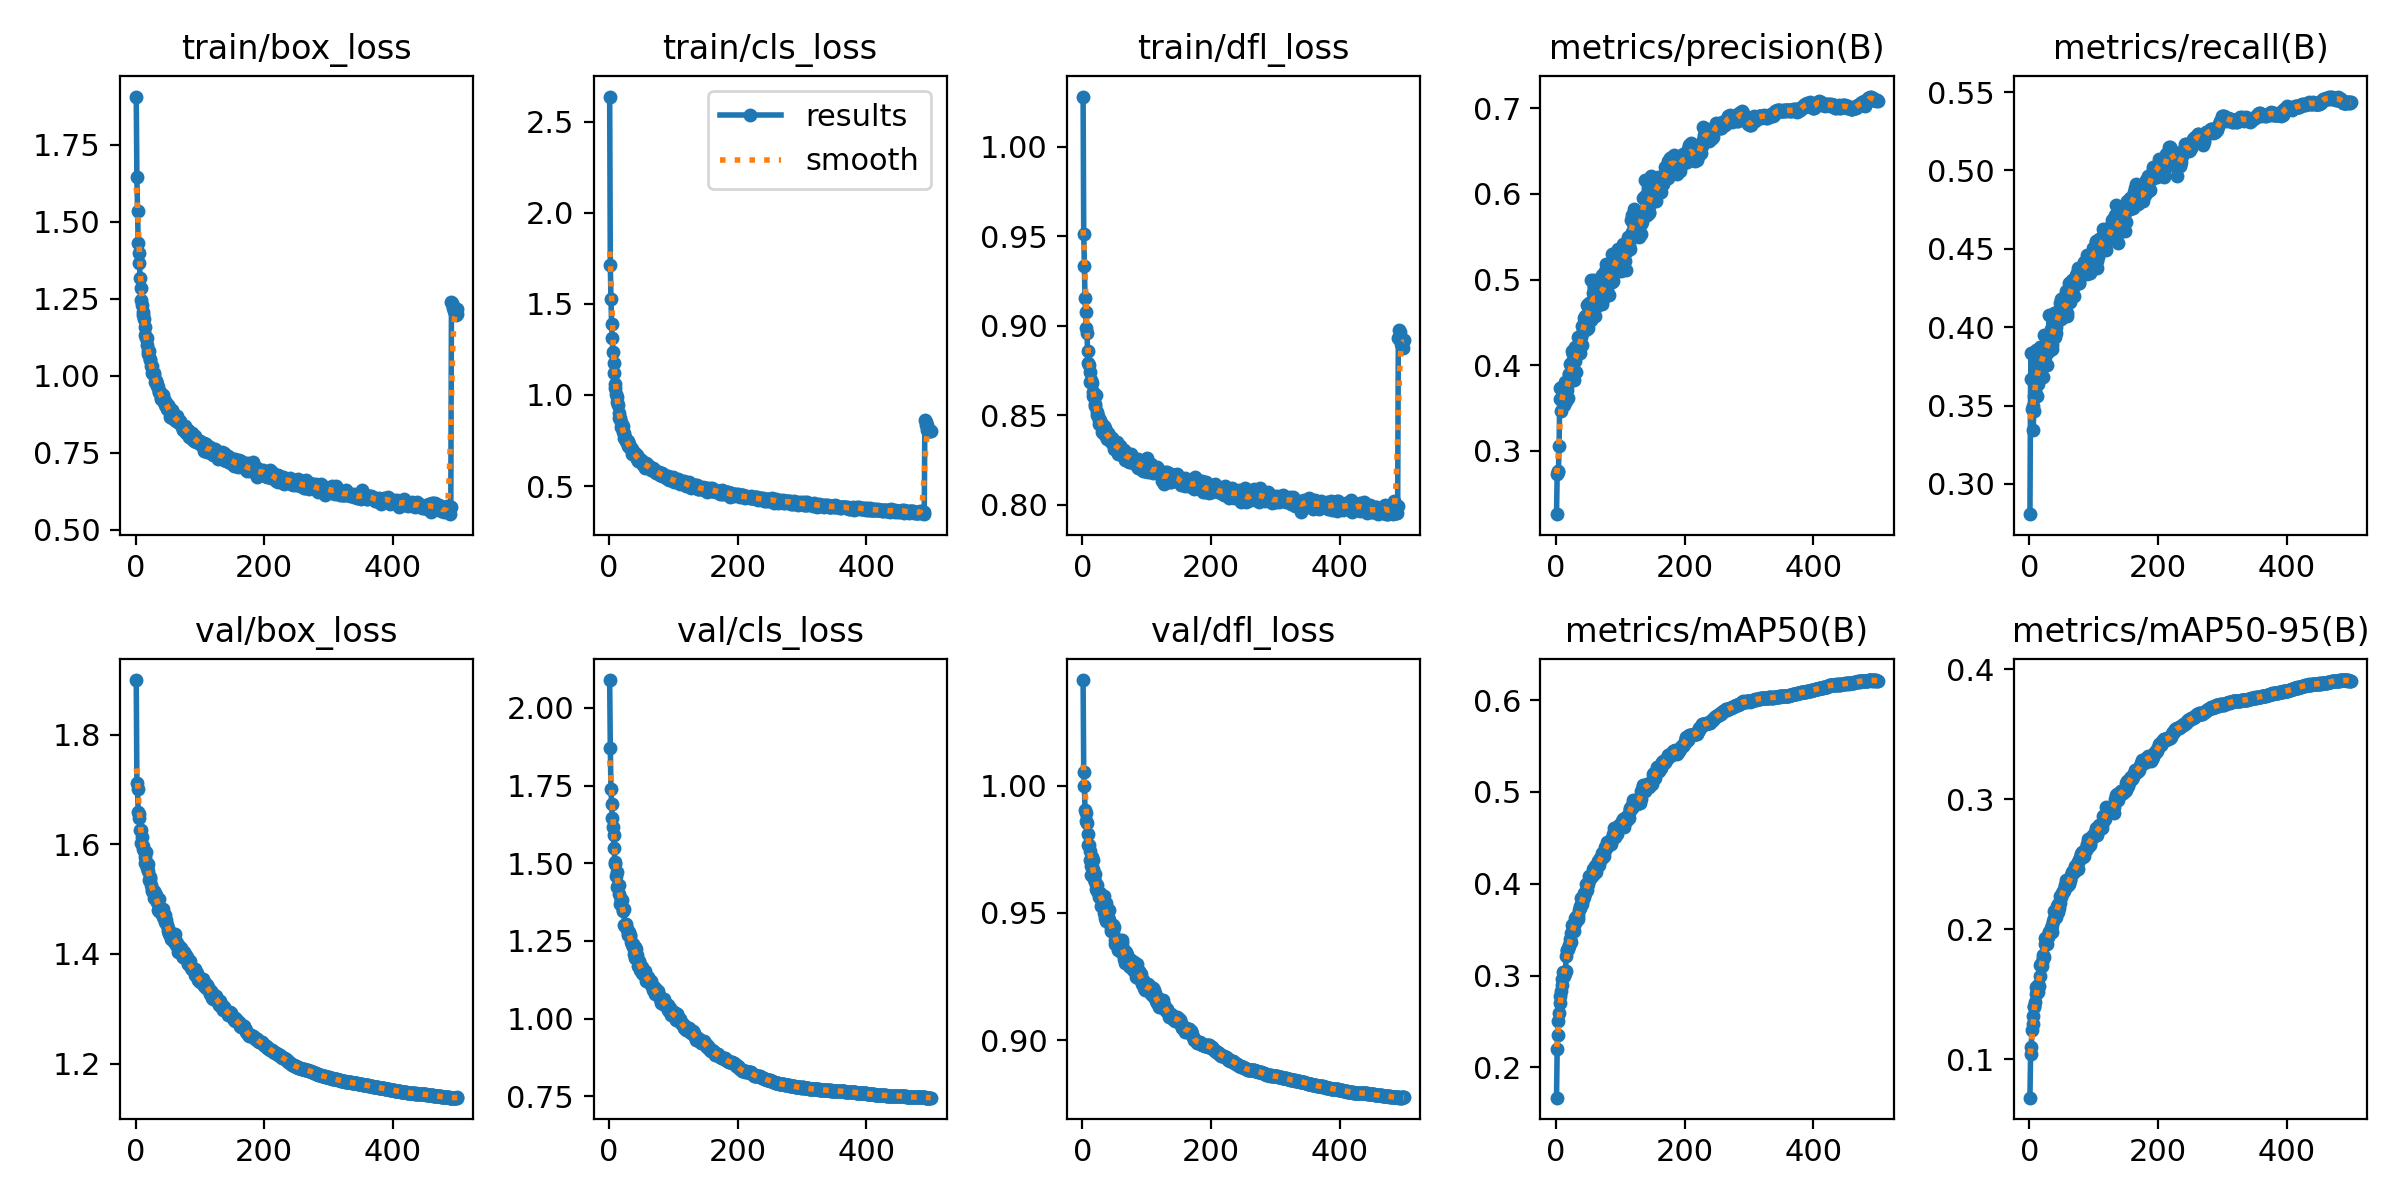
\includegraphics[width=0.8\textwidth]{v_2/small-1202/results.png}
    \caption{Andamento funzioni di loss e metriche durante l'esecuzione di v8m12}
    \label{fig:v2-1}
\end{figure}

% Dettagli configurazione, tipologia modello e iperparametri, dove è stato eseguito il train

% Risultati training
    % - andamento training
    % - grafici recall e precision e performance e F1
    % - matrici di confusione
    % - tabella performance test set

% Commento risultati

primo modello